\documentclass[pdflatex,sn-mathphys-num,iicol]{sn-jnl}

\usepackage{bookmark}
\usepackage{tabularx}
\usepackage{tikz}
\usetikzlibrary{shapes.geometric, shapes.misc, arrows.meta, positioning, calc}
\usepackage{graphicx}
\usepackage{mwe}
\usepackage{multirow}
\usepackage{amsmath,amssymb,amsfonts}
\usepackage{amsthm}
\usepackage{mathrsfs}
\usepackage[title]{appendix}
\usepackage{xcolor}
\usepackage{textcomp}
\usepackage{manyfoot}
\usepackage{booktabs}

\theoremstyle{thmstyleone}
\newtheorem{theorem}{Theorem}
\newtheorem{proposition}[theorem]{Proposition}
\theoremstyle{thmstyletwo}
\newtheorem{example}{Example}
\newtheorem{remark}{Remark}
\theoremstyle{thmstylethree}
\newtheorem{definition}{Definition}

\raggedbottom

\begin{document}

\title[Which Shift Costs a CQT--CNN the Most]{Which Acoustic Shift Costs a CQT--CNN the Most? A Seed-Level Ablation on Isolated Piano Chords}

\author*[1]{\fnm{Cikal} \sur{Gemintang Seya}}\email{cikalgemintangseya1@gmail.com}

\author[1]{\fnm{Jasman} \sur{Pardede}}\email{jasman@itenas.ac.id}

\affil*[1]{\orgdiv{Informatics}, \orgname{National Institute of Technology}, \orgaddress{\street{Neglasari}, \city{Bandung}, \postcode{40124}, \state{West Java}, \country{Indonesia}}}

\abstract{Isolated piano-chord audio is a 36-class recognition problem: 12 roots $\times$ three interval templates (major, minor, diminished). We train a compact Convolutional Neural Network (CNN) on Constant-Q Transform (CQT) features from a Techno T-9890i keyboard and evaluate it without fine-tuning under two recorded factors -- recording-setting shift (same keyboard, three other microphones) and keyboard shift (a Yamaha PSR-S910 on two of those recording setups) -- then under eval-only interior noise. The architecture is retrained ten times: five seeds on the full 7{,}200-clip training set (\texttt{orig}) and five seeds after dropping sixteen silent clips (\texttt{clean}). In-domain accuracy stays at or above 0.999 for every run. Out of domain the ordering is stable across both variants and all ten seeds: a new microphone on the Techno is cheaper than a new keyboard on a matched recording setup, and eval-only ESC-50 noise then compounds the keyboard cost. The silent-clip ablation is not a free improvement. \texttt{clean} seed 42 falls to 0.348 / 0.368 on the two Yamaha datasets while the matching \texttt{orig} seed stays at 0.963 / 0.961; other \texttt{clean} seeds are mixed. A single seed can invert the apparent value of the data-quality fix and can shrink or inflate the keyboard gap by tens of points. We therefore report every seed.}

\keywords{Constant-Q Transform, Convolutional Neural Network, domain shift, ablation, seed variance}

\maketitle

\section{Introduction}\label{sec1}

Recognizing musical chords directly from raw audio is a foundational task in music information retrieval (MIR), underpinning applications such as automatic music transcription, interactive music education tools, and real-time performance feedback systems \cite{Telila2023}\cite{Saputra2021}\cite{Moysis2023}. Unlike symbolic or MIDI-based chord recognition, audio-based recognition must contend with the acoustic realities of sound production: a chord played on one instrument, in one room, captured by one microphone, does not produce the same waveform as the identical chord played on a different instrument, in a different room, captured by a different microphone. This variability is the central obstacle to deploying chord recognition systems in real-world settings, where the recording conditions encountered at inference time are rarely identical to those under which a model was trained \cite{Kusaka2024}.

This mismatch is termed acoustic domain shift and is driven by at least three factors: keyboard variation, where a different instrument's voice synthesis displaces chord vectors in feature space; environmental shift, where room acoustics and ambient noise absent during training move the acoustic scene; and recording-setting shift, where a different microphone, its placement, and its on-device signal chain -- codec, gain, or built-in processing, not the transducer's frequency response alone -- change the captured spectrum \cite{Kusaka2024}\cite{Majchrzak2025}. Classification errors under domain shift are not a symptom of insufficient training data: each factor moves the test feature distribution away from the one the classifier was optimized on.

A joint shift matches deployment, but one number hides the cause. A phone microphone on the Techno T-9890i and the Yamaha PSR-S910 on a laptop microphone already used for a recording-setting test are different problems, and neither is a noisy room. Isolating them with independently recorded datasets, then matching environment with a controlled synthetic overlay, is needed before ranking the factors.

Time-frequency representations that convert audio into image-like matrices, classified with convolutional architectures, are the dominant paradigm across audio recognition tasks \cite{Wolf-Monheim2025}\cite{Zaman2023}\cite{Moysis2023}. Among these, the Constant-Q Transform (CQT) suits keyboard and chord audio: unlike the Short-Time Fourier Transform's linearly spaced bins, CQT bins are logarithmically spaced at a constant quality factor, aligning each bin with a musical semitone \cite{Lacoste2007}, so a transposition is a vertical shift and harmonic intervals keep a consistent shape \cite{Li2021}. Li \cite{Li2021} reported 84.2\% accuracy for CQT-based chord recognition versus 75.3\% for STFT and 80.8\% for CENS chromagrams under identical CNN architectures; Telila et al.\ \cite{Telila2023} and O'Hanlon and Sandler \cite{OHanlon2021} report comparable gains from the same alignment. We keep CQT as the input.

The piano chord problem provides a controlled vocabulary for generalization analysis. With 36 classes formed by 12 chromatic roots and 3 qualities (major, minor, diminished), the task requires fine-grained spectral discrimination: major and minor triads differ by a semitone shift in the third, diminished triads by a further semitone in the fifth \cite{Harte2010}. A CNN's convolutional kernels respond to small time-frequency neighborhoods \cite{OShea2015}\cite{Purwono2022}, so local interval geometry can survive a global envelope shift from a new microphone or piano voice.

Edwards et al.\ \cite{Edwards2024} run the closest controlled piano out-of-domain (OOD) study, on note-level transcription rather than chords: they re-record MAESTRO on a Yamaha Disklavier, evaluate on MAPS, and degrade test audio with noise, EQ, pitch shift, and reverb. A studio-only model overfits that room; train-time mixing recovers 88.4 MAPS note-onset F1 with no MAPS training audio. Kusaka and Maezawa \cite{Kusaka2024} use a related recipe for mobile automatic music transcription. Both treat augmentation as a training intervention; we keep the opposite protocol -- a clean-trained CQT--CNN, recorded and synthetic shifts only at evaluation -- so each factor's cost is visible before anyone mixes the training set.

Chord papers still grow the vocabulary \cite{Majchrzak2025} or swap in conformers \cite{Akram2025} and attention \cite{Kusaka2024}, test in-domain, and treat OOD conditions as missing data to be patched with synthetic audio \cite{Byambatsogt2020}\cite{Ostermann2023}. What is missing on isolated piano chords is a factorized reading of a CQT--CNN that also says whether a training-set defect changes the ranking: sixteen digital-silence clips sit in the Techno training set, 8\% of one class. Dropping them looks like an obvious fix. Whether it changes which shift costs the most, and whether that answer depends on the seed, is an empirical question. In-domain accuracy saturates at 1.00 and cannot answer it. We therefore retrain the same architecture ten times -- five seeds with the silent clips (\texttt{orig}), five seeds without them (\texttt{clean}) -- and report every seed on every held-out condition.

Contributions:
\begin{enumerate}[1.]
\item A Techno T-9890i training set and five held-out datasets -- three recording-setting-shift datasets (one, \texttt{vivo}, without a keyboard-shift counterpart) and two Yamaha PSR-S910 keyboard-shift datasets on recording setups already used for the recording-setting tests.
\item Shared CQT features ($216\times188\times1$) and a compact CNN, retrained under two training-set configurations $\times$ five seeds.
\item Frozen-weight evaluation that isolates recording-setting change from keyboard change, then adds eval-only ESC-50 interior noise, with every seed listed rather than only a mean and a range.
\item A ranking of those factors: keyboard shift is the largest recorded cost on every seed of both variants; noise then compounds it; dropping the silent clips does not remove that ordering and can make one seed collapse on the Yamaha sets.
\end{enumerate}

\section{Methodology}\label{sec3}

Fig.~\ref{fig:methodology} shows the pipeline: dataset acquisition, CQT extraction, the \texttt{orig}/\texttt{clean} $\times$ 5-seed CNN retrain, recorded OOD evaluation, and eval-only noise. Software: Python 3.10, TensorFlow 2.15, scikit-learn 1.7.2, Librosa 0.11.0, NumPy 1.26.4, Matplotlib 3.10.8. Hardware: ASUS ROG Flow X13 (Ryzen 7 6800HS, RTX 3050 Ti, 16\,GB RAM), an RTX 2080 Ti eGPU for the retrain batch, and Google Colaboratory (T4/A100).

\begin{figure}[t]
  \centering
  \resizebox{0.92\columnwidth}{!}{%
  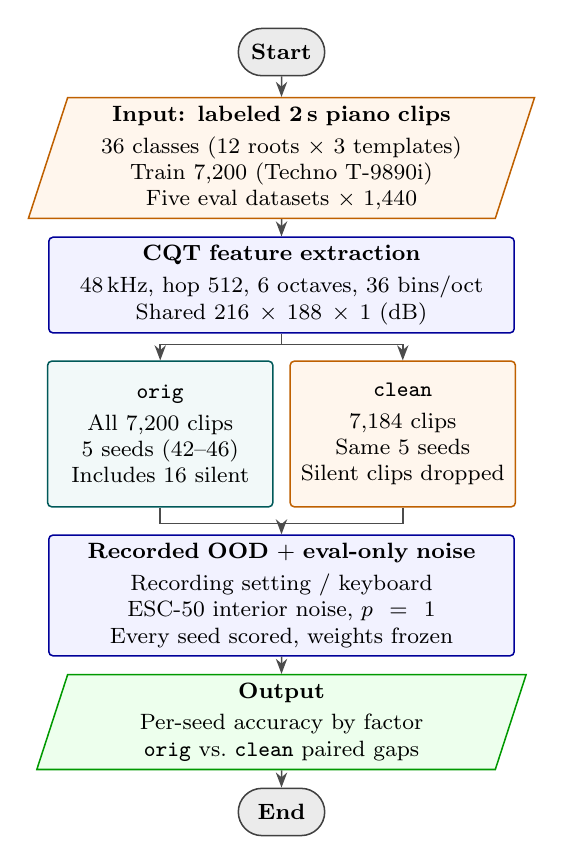
\begin{tikzpicture}[
    node distance=0.16cm and 0.10cm,
    >={Stealth},
    font=\footnotesize,
    base/.style={draw, align=center, minimum height=0.52cm, line width=0.55pt, inner sep=3pt},
    terminal/.style={base, shape=rounded rectangle, rounded rectangle arc length=180, draw=black!75, fill=black!8, minimum height=0.60cm, minimum width=1.8cm, inner xsep=10pt, inner ysep=2pt, font=\footnotesize\bfseries},
    process/.style={base, rectangle, rounded corners=1.5pt, draw=blue!60!black, fill=blue!5, text width=5.7cm},
    orig/.style={base, rectangle, rounded corners=1.5pt, draw=teal!70!black, fill=teal!5, text width=2.65cm, minimum height=1.85cm},
    clean/.style={base, rectangle, rounded corners=1.5pt, draw=orange!75!black, fill=orange!7, text width=2.65cm, minimum height=1.85cm},
    io/.style={base, trapezium, trapezium left angle=72, trapezium right angle=108, trapezium stretches body=true, draw=orange!75!black, fill=orange!7, text width=5.15cm, inner xsep=4pt},
    result/.style={base, trapezium, trapezium left angle=72, trapezium right angle=108, trapezium stretches body=true, draw=green!60!black, fill=green!7, text width=5.15cm, inner xsep=4pt},
    arrow/.style={->, line width=0.55pt, black!70}
  ]
    \node[terminal] (start) {Start};
    \node[io, below=0.26cm of start] (in1)
    {\textbf{Input: labeled 2\,s piano clips}\\[2pt]
     36 classes (12 roots $\times$ 3 templates)\\
     Train 7{,}200 (Techno T-9890i)\\
     Five eval datasets $\times$ 1{,}440};
    \node[process, below=0.22cm of in1] (p2)
    {\textbf{CQT feature extraction}\\[2pt]
     48\,kHz, hop 512, 6 octaves, 36 bins/oct\\
     Shared $216 \times 188 \times 1$ (dB)};
    \node[orig, below left=0.34cm and 0.10cm of p2.south, anchor=north east] (o1)
    {\textbf{\texttt{orig}}\\[2pt]
     All 7{,}200 clips\\
     5 seeds (42--46)\\
     Includes 16 silent};
    \node[clean, below right=0.34cm and 0.10cm of p2.south, anchor=north west] (c1)
    {\textbf{\texttt{clean}}\\[2pt]
     7{,}184 clips\\
     Same 5 seeds\\
     Silent clips dropped};
    \node[process, below=0.34cm of $(o1.south)!0.5!(c1.south)$, anchor=north] (p5)
    {\textbf{Recorded OOD $+$ eval-only noise}\\[2pt]
     Recording setting / keyboard\\
     ESC-50 interior noise, $p=1$\\
     Every seed scored, weights frozen};
    \node[result, below=0.22cm of p5] (out)
    {\textbf{Output}\\[2pt]
     Per-seed accuracy by factor\\
     \texttt{orig} vs.\ \texttt{clean} paired gaps};
    \node[terminal, below=0.22cm of out] (endn) {End};
    \draw[arrow] (start) -- (in1);
    \draw[arrow] (in1) -- (p2);
    \draw[arrow] (p2.south) -- ++(0,-0.14) -| (o1.north);
    \draw[arrow] (p2.south) -- ++(0,-0.14) -| (c1.north);
    \coordinate (merge) at ($(p5.north)+(0,0.14)$);
    \draw[line width=0.55pt, black!70] (o1.south) |- (merge);
    \draw[line width=0.55pt, black!70] (c1.south) |- (merge);
    \draw[arrow] (merge) -- (p5.north);
    \draw[arrow] (p5) -- (out);
    \draw[arrow] (out) -- (endn);
  \end{tikzpicture}%
  }
  \caption{Experimental pipeline. Shared CQT features feed two training-set variants $\times$ five seeds. Overlays hit evaluation datasets only; CNN weights stay frozen after training.}
  \label{fig:methodology}
\end{figure}

\subsection{Two evaluation scenarios}\label{subsec3_0}

Scenario~1 (in-domain) holds instrument, room, and recording setting fixed and asks whether the CQT space separates the 36 classes at all. Five-fold cross-validation on the 7{,}200 Techno takes measures this for the reference architecture; each retrain below also reports its own held-out Techno test split.

Scenario~2 changes one factor at a time and tests each trained CNN checkpoint with no fine-tuning. Three recording-setting-shift datasets keep the Techno T-9890i and change the recording setup -- microphone, placement, and on-device signal chain, not the transducer alone (ThinkPad P14s Gen 2 Intel internal mic, Vivo Y27s phone, ASUS ROG Flow X13 2022 internal mic). Two keyboard-shift datasets then swap the instrument to a Yamaha PSR-S910 while reusing the ThinkPad and Flow recording setups already measured on the Techno. That pairing is the point: \texttt{thinkpad} versus \texttt{thinkpad-2} differs by keyboard, not by recording setup; \texttt{flow} versus \texttt{flow-2} does the same. \texttt{vivo} has no Yamaha counterpart, so it contributes recording-setting-shift evidence but not a matched pair. Table~\ref{tab:scenarios} lists every dataset. Eval-only noise (Section~\ref{subsec3_7}) hits all five 1{,}440-sample datasets. No checkpoint is fine-tuned on evaluation data.

\begin{table*}[t]
\caption{Recorded evaluation datasets. The CNN is trained on \texttt{training} and evaluated on every dataset. $^\dagger$\texttt{vivo} has no Yamaha counterpart.}\label{tab:scenarios}
\begin{tabular*}{\textwidth}{@{\extracolsep{\fill}}lllll@{}}
\toprule
Dataset & $N$ & Primary shift & Instrument & Recording setting \\
\midrule
\texttt{training} & 7{,}200 & None (in-domain) & Techno T-9890i & Xiaomi Redmi Pad 2 \\
\texttt{thinkpad} & 1{,}440 & Recording setting & Techno T-9890i & ThinkPad P14s Gen 2 (Intel) \\
\texttt{vivo} & 1{,}440 & Recording setting$^\dagger$ & Techno T-9890i & Vivo Y27s \\
\texttt{flow} & 1{,}440 & Recording setting & Techno T-9890i & ASUS ROG Flow X13 (2022) \\
\texttt{thinkpad-2} & 1{,}440 & Keyboard & Yamaha PSR-S910 & ThinkPad P14s Gen 2 (Intel) \\
\texttt{flow-2} & 1{,}440 & Keyboard & Yamaha PSR-S910 & ASUS ROG Flow X13 (2022) \\
\bottomrule
\end{tabular*}
\end{table*}

\subsection{Dataset acquisition}\label{subsec3_1}

A web recorder sends simultaneous MIDI note-on events over USB and captures the microphone. That removes manual playing errors and keeps the instrument's physical resonance and synthesis. The same trigger list and voicing are used for every dataset, so class identity does not change with the acoustic condition.

The vocabulary is 36 classes. Each class is a three-note piano sound: one of 12 roots (C, C$\sharp$, \ldots, B) times one of three interval templates (maj $+4,+3$; min $+3,+4$; dim $+3,+3$ semitones). A semitone is one chromatic step and occupies three CQT bins. Figures write \emph{C maj}, \emph{E dim}; file names keep the fourth-octave suffix. All takes sit in that octave, inside C1--C7 ($\approx$33--2093\,Hz) \cite{Telila2023}\cite{Harte2010}. The dim template places its three notes closer together than maj or min \cite{Byambatsogt2020}. Both instruments use a grand-piano preset; they still differ in sample set, loudspeaker, and cabinet.

\begin{enumerate}[1.]
\item \textbf{Training (\texttt{training})}: 200 samples per class, 7{,}200 total. Xiaomi Redmi Pad 2 mic, Techno T-9890i Acoustic Grand Piano. Attack delays 0--150\,ms approximate keystroke asynchrony \cite{Bella2011}. OGG/OPUS, 48{,}000\,Hz, 32-bit, mono, no filters. Sixteen clips (8\% of $C$ diminished, a recorder fault) are digital silence. Section~\ref{subsec3_variants} trains with and without them.
\item \textbf{Recording-setting shift (\texttt{thinkpad}, \texttt{vivo}, \texttt{flow})}: 40 per class, 1{,}440 each, WAV. Techno T-9890i on the ThinkPad P14s Gen 2 (Intel) internal mic, a Vivo Y27s phone mic, and the ASUS ROG Flow X13 (2022) internal mic.
\item \textbf{Keyboard shift (\texttt{thinkpad-2}, \texttt{flow-2})}: 40 per class, 1{,}440 each, WAV. Yamaha PSR-S910 on the ThinkPad and Flow recording setups already used on the Techno.
\end{enumerate}

No evaluation clip enters training, validation, early stopping, or hyperparameter choice.

\subsection{CQT feature extraction}\label{subsec3_2}

We compute CQT with \texttt{librosa.cqt()}. Each bin $f_k$ has constant quality
\begin{equation}
Q = \frac{f_k}{f_{k+1} - f_k} = \frac{1}{2^{1/B} - 1}
\label{eq:cqt}
\end{equation}
where $B$ is bins per octave \cite{Li2021}\cite{Lacoste2007}. Logarithmic spacing lines bins up with semitones, so a transposition is a vertical shift and a major third is the same bin distance on every root \cite{Harte2010}.

Table~\ref{tab:cqt-extraction-params} lists parameters. Thirty-six bins per octave (3 per semitone) resolve major ($+4,+3$), minor ($+3,+4$), and diminished ($+3,+3$) intervals \cite{Akram2025}\cite{OHanlon2021}. Each clip is truncated to a fixed 2.0\,s. Equation~\ref{eq:frames} gives 188 frames and a uniform shape $216 \times 188 \times 1$. Magnitudes go to dB with \texttt{librosa.amplitude\_to\_db(..., ref=np.max)}. The same parameters are used for training, every recorded dataset, and the noise overlay.

\begin{equation}
\text{frames} = \frac{\text{duration} \times \text{sample rate}}{\text{hop size}}
\label{eq:frames}
\end{equation}

\begin{table}[t]
\caption{CQT feature extraction parameters}\label{tab:cqt-extraction-params}
\begin{tabular}{@{}ll@{}}
\toprule
Parameter & Value \\
\midrule
Sample rate & 48{,}000\,Hz \\
Hop size & 512 samples \\
Octaves & 6 \\
Bins per octave & 36 \\
Total bins & 216 \\
Frequency range & C1 (32.70\,Hz) to C7 (2{,}093\,Hz) \\
Window & Hann \\
Frame length & 188 \\
Output shape & $216 \times 188 \times 1$ \\
\bottomrule
\end{tabular}
\end{table}

\begin{figure}[t]
\centering
\includegraphics[width=\columnwidth]{fig-cqt-train.png}
\caption{Training CQT of C maj ($+4,+3$) and C min ($+3,+4$): same root, one-semitone gap in the middle note. Frequency in Hz.}
\label{fig:cqt-spectrograms}
\end{figure}

\subsection{CNN architecture and training}\label{subsec3_3}

The CNN follows Wolf-Monheim \cite{Wolf-Monheim2025}, originally designed for environmental sound classification on ESC-50. Its compact four-block convolutional structure without recurrent layers or attention is appropriate for fixed-window classification from static spectrograms.

Table~\ref{tab:cnn-architecture} lists layers. Input batch normalization fits its scale and shift to the training distribution once and applies that fixed transform to every clip at inference. The four Conv2D--MaxPooling2D blocks build a progressive hierarchy: the first block (64 filters) captures low-level spectral texture; the second (128 filters) encodes mid-level harmonic interval patterns; the third and fourth (256 filters each) represent chord-quality abstractions. The $3\times3$ receptive field matches the 1--2 bin frequency shifts that distinguish chord types, while MaxPooling provides spatial subsampling and limited translation invariance \cite{Purwono2022}. Dropout (rate 0.5) limits co-adaptation to the Techno piano voice.

\begin{table}[t]
\caption{CNN architecture specification}\label{tab:cnn-architecture}
\begin{tabularx}{\columnwidth}{@{}lXl@{}}
\toprule
Layer & Output shape & Notes \\
\midrule
BatchNorm & $216{\times}188{\times}1$ & Input normalization \\
Conv2D & $216{\times}188{\times}64$ & $3{\times}3$, ReLU, same \\
MaxPool & $108{\times}94{\times}64$ & $2{\times}2$, stride 2 \\
Conv2D & $108{\times}94{\times}128$ & $3{\times}3$, ReLU, same \\
MaxPool & $54{\times}47{\times}128$ & $2{\times}2$, stride 2 \\
Conv2D & $54{\times}47{\times}256$ & $3{\times}3$, ReLU, same \\
MaxPool & $27{\times}23{\times}256$ & $2{\times}2$, stride 2 \\
Conv2D & $27{\times}23{\times}256$ & $3{\times}3$, ReLU, same \\
MaxPool & $13{\times}11{\times}256$ & $2{\times}2$, stride 2 \\
Flatten & 36{,}608 & \\
Dense & 256 & ReLU \\
Dropout & 256 & rate 0.5 \\
Dense & 36 & Softmax \\
\bottomrule
\end{tabularx}
\end{table}

Training follows Table~\ref{tab:cnn-training-config}. Stratified 80/10/10 sampling keeps class balance. The seed is reused for the split, the weight initialization, and TensorFlow's global RNG. \texttt{ReduceLROnPlateau} multiplies the learning rate by 0.1 after 2 stagnant val-loss epochs; \texttt{EarlyStopping} stops after 6; max 50 epochs \cite{Wolf-Monheim2025}. The 10\% test split is held out of training and validation.

\begin{table}[t]
\caption{CNN training configuration}\label{tab:cnn-training-config}
\begin{tabular}{@{}ll@{}}
\toprule
Parameter & Value \\
\midrule
Seeds & 42, 43, 44, 45, 46 \\
Train / Val / Test split & 80\% / 10\% / 10\% \\
Batch size & 32 \\
Initial learning rate & 0.001 \\
Optimizer & Adam \\
Weight initialization & Glorot uniform \\
Loss & Categorical cross-entropy \\
Max epochs & 50 \\
EarlyStopping patience & 6 epochs \\
ReduceLROnPlateau & factor 0.1, patience 2 \\
\bottomrule
\end{tabular}
\end{table}

\subsection{5-fold cross-validation}\label{subsec3_5}

Five folds on all 7{,}200 training samples, 80/20 per fold, measure in-domain score independent of one train/test split. Each fold retrains the CNN from a fresh random initialization and a fixed per-fold seed. Fold test partitions never enter training or early stopping for that fold.

\subsection{Training-set ablation}\label{subsec3_variants}

Two training configurations share Table~\ref{tab:cnn-architecture} and Table~\ref{tab:cnn-training-config}. \texttt{orig} uses all 7{,}200 clips, including the sixteen silent $C$ diminished takes. \texttt{clean} drops those sixteen clips (7{,}184 remaining) and otherwise matches \texttt{orig}. Each configuration is retrained from seeds 42--46, producing ten checkpoints. The only intended difference between a paired \texttt{orig} and \texttt{clean} run of the same seed is the presence of those sixteen clips in the training pool and the resulting train/validation/test split. No other hyperparameter is changed.

\subsection{Eval-only noise}\label{subsec3_7}

Additive interior noise hits already out-of-domain datasets without retraining, applied to all ten checkpoints. ESC-50 interior/domestic clips \cite{Piczak2015} are converted to CQT with the same hop and binning as the chord features, yielding a 400-clip bank over 10 classes. Mixing is performed in the CQT power domain at a uniform SNR drawn from $[10, 25]$\,dB (realized mean 17.5\,dB) with a random time roll. Overlay probability is 1 (every evaluation sample is degraded), the draw is random per sample with a fixed seed, and wet features are not written back into the training tree. This is a controlled interior overlay, not a claim that ESC-50 matches any one room. Indoor room impulse responses and measured microphone impulse responses were applied under the same eval-only rule; they are not the primary ranking below.

\subsection{Evaluation metrics}\label{subsec3_6}

Accuracy is the fraction of clips with the correct label. Precision, recall, and F1 for a one-versus-rest partition of a single class are
\begin{equation}
\mathrm{P}=\frac{\mathrm{TP}}{\mathrm{TP}+\mathrm{FP}},\quad
\mathrm{R}=\frac{\mathrm{TP}}{\mathrm{TP}+\mathrm{FN}},\quad
\mathrm{F1}=\frac{2\mathrm{PR}}{\mathrm{P}+\mathrm{R}}.
\label{eq:prf}
\end{equation}
Macro P, R, and F1 are unweighted means over the 36 classes. Headline tables report accuracy per seed. A paired keyboard gap is the recording-setting accuracy minus the matched keyboard-shift accuracy on the same checkpoint (\texttt{thinkpad} minus \texttt{thinkpad-2}; \texttt{flow} minus \texttt{flow-2}). A noise tax is recorded accuracy minus noise accuracy on the same checkpoint and dataset.

\section{Results}\label{sec4}

\subsection{CQT feature extraction}\label{subsec4_1}

Every clip becomes a $216 \times 188$ CQT dB matrix. Fig.~\ref{fig:cqt-spectrograms} shows C maj and C min from the training set: same root, one semitone (three CQT bins) in the middle note.

\subsection{In-domain performance}\label{subsec4_2}

Under Scenario~1 the CNN scores 1.00 accuracy, precision, recall, and F1 on every fold of the 7{,}200 Techno takes. On the held-out Techno test split of the ten retrains, every \texttt{orig} seed is 1.000; \texttt{clean} seeds 42, 44, 45, and 46 are 1.000 and seed 43 is 0.999. Resubstitution on the full training dataset is 0.9999: one $C$ diminished clip is predicted $C$ minor. With instrument, room, and recording setting fixed, the CQT space separates the 36 classes for both training-set variants. That result does not rank the OOD factors.

\subsection{Recorded out-of-domain evaluation, every seed}\label{subsec4_3}

Table~\ref{tab:seeds-recorded} lists accuracy for each seed on each held-out recording. Fig.~\ref{fig:cross-domain} summarizes the same comparison.

On \texttt{orig}, recording-setting means are 0.961 (\texttt{thinkpad}), 0.903 (\texttt{vivo}), and 0.911 (\texttt{flow}). Keyboard means are 0.803 (\texttt{thinkpad-2}) and 0.815 (\texttt{flow-2}). The cheapest OOD cell is \texttt{orig} seed 42 on \texttt{vivo} (0.999) and on \texttt{thinkpad} (0.999); the dearest recorded cells for \texttt{orig} are seed 45 on \texttt{thinkpad-2} (0.705) and seed 43 on \texttt{thinkpad-2} (0.719) and \texttt{flow-2} (0.720). Seed 42 is the most robust \texttt{orig} run (Yamaha 0.963 / 0.961). Seed 45 is the weakest on four of the five datasets.

On \texttt{clean} the recording-setting means are close to \texttt{orig}: 0.962, 0.894, 0.900. The keyboard means fall to 0.719 and 0.728, pulled down by seed 42 (0.348 on \texttt{thinkpad-2}, 0.368 on \texttt{flow-2}). The same seed is not weak on Techno: 0.985 / 0.884 / 0.831. Other \texttt{clean} seeds do not repeat that collapse. Seed 44 is the strongest \texttt{clean} Yamaha run (0.925 / 0.935). Seed 43 is the weakest recording-setting run (0.857 / 0.742 / 0.810) without being the weakest keyboard run.

Dropping the silent clips therefore does not produce a uniformly better OOD model. Relative to the paired \texttt{orig} seed, \texttt{clean} is better on some dataset--seed cells (seed 45 on every dataset; seed 44 on four of five) and worse on others (seed 42 on every dataset; seed 43 on four of five). The mean keyboard gap is larger under \texttt{clean} because of seed 42.

\begin{table*}[t]
\caption{Out-of-domain accuracy by seed. \texttt{orig}: trained on 7{,}200 clips. \texttt{clean}: sixteen silent clips removed.}\label{tab:seeds-recorded}
\setlength{\tabcolsep}{4pt}
\begin{tabular*}{\textwidth}{@{\extracolsep{\fill}}llcccccc@{}}
\toprule
Variant & Dataset & 42 & 43 & 44 & 45 & 46 & Mean \\
\midrule
\texttt{orig} & \texttt{thinkpad} & 0.999 & 0.967 & 0.958 & 0.895 & 0.984 & 0.961 \\
\texttt{orig} & \texttt{vivo} & 0.999 & 0.896 & 0.883 & 0.776 & 0.960 & 0.903 \\
\texttt{orig} & \texttt{flow} & 0.994 & 0.863 & 0.940 & 0.801 & 0.958 & 0.911 \\
\texttt{orig} & \texttt{thinkpad-2} & 0.963 & 0.719 & 0.847 & 0.705 & 0.780 & 0.803 \\
\texttt{orig} & \texttt{flow-2} & 0.961 & 0.720 & 0.842 & 0.740 & 0.810 & 0.815 \\
\midrule
\texttt{clean} & \texttt{thinkpad} & 0.985 & 0.857 & 0.975 & 0.999 & 0.996 & 0.962 \\
\texttt{clean} & \texttt{vivo} & 0.884 & 0.742 & 0.971 & 0.997 & 0.879 & 0.894 \\
\texttt{clean} & \texttt{flow} & 0.831 & 0.810 & 0.981 & 0.988 & 0.891 & 0.900 \\
\texttt{clean} & \texttt{thinkpad-2} & 0.348 & 0.698 & 0.925 & 0.884 & 0.740 & 0.719 \\
\texttt{clean} & \texttt{flow-2} & 0.368 & 0.685 & 0.935 & 0.903 & 0.749 & 0.728 \\
\bottomrule
\end{tabular*}
\end{table*}

\begin{figure}[htbp]
\centering
\includegraphics[width=\columnwidth,height=0.26\textheight,keepaspectratio]{fig-cross-domain.pdf}
\caption{Recorded out-of-domain accuracy for \texttt{orig} and \texttt{clean}. Open markers are the five seeds; filled markers are the mean $\pm$ sd. Per-seed values are in Table~\ref{tab:seeds-recorded}.}
\label{fig:cross-domain}
\end{figure}

\subsection{Which recorded factor costs more, seed by seed}\label{subsec4_3b}

Table~\ref{tab:paired} converts Table~\ref{tab:seeds-recorded} into the two matched-pair gaps that isolate the keyboard. Every one of the ten checkpoints loses accuracy when the keyboard changes and the recording setup does not. The gap is never zero and never negative.

On \texttt{orig} the ThinkPad keyboard gap is 3.6, 24.8, 11.1, 19.0, and 20.4 points across seeds 42--46; the Flow gap is 3.3, 14.2, 9.8, 6.0, and 14.7 points. Seed 42, the strongest OOD run, still pays a keyboard tax, just a small one. Seed 43 pays the largest ThinkPad tax (24.8 points) and a 14.2-point Flow tax.

On \texttt{clean} the ThinkPad gaps are 63.7, 15.9, 5.0, 11.5, and 25.6 points; the Flow gaps are 46.3, 12.6, 4.6, 8.5, and 14.2 points. Seed 42 dominates the mean. Remove that seed and the remaining \texttt{clean} gaps sit in the same band as \texttt{orig}. The ablation leaves the factor ranking in place and changes how expensive the keyboard looks for one initialization.

Recording-setting shift itself is not free. Against in-domain 1.00, \texttt{orig} seed 45 already sits at 0.895 / 0.776 / 0.801 on the three Techno OOD sets. That is a microphone-and-chain cost of 10--22 points with the keyboard held fixed. It is still smaller, on that same seed, than the additional keyboard cost on ThinkPad (19.0 points) and comparable to the Flow keyboard cost (6.0 points). Across the ten checkpoints, the largest single recorded drop from a matched Techno baseline is the \texttt{clean} seed-42 keyboard swap.

\begin{table}[htbp]
\caption{Paired keyboard gap in accuracy points: recording-setting minus matched Yamaha, same checkpoint. All ten values are positive.}\label{tab:paired}
\setlength{\tabcolsep}{3.5pt}
\begin{tabular}{@{}llccccc@{}}
\toprule
Variant & Pair & 42 & 43 & 44 & 45 & 46 \\
\midrule
\texttt{orig} & ThinkPad & 3.6 & 24.8 & 11.1 & 19.0 & 20.4 \\
\texttt{orig} & Flow & 3.3 & 14.2 & 9.8 & 6.0 & 14.7 \\
\texttt{clean} & ThinkPad & 63.7 & 15.9 & 5.0 & 11.5 & 25.6 \\
\texttt{clean} & Flow & 46.3 & 12.6 & 4.6 & 8.5 & 14.2 \\
\bottomrule
\end{tabular}
\end{table}

\subsection{Eval-only noise, every seed}\label{subsec4_4}

Table~\ref{tab:seeds-noise} lists accuracy after ESC-50 interior noise is mixed into every evaluation clip. Fig.~\ref{fig:aug} summarizes the overlay comparison.

Noise lowers accuracy on all 50 dataset--seed cells of both variants. On \texttt{orig} the mean tax is 10.2, 7.6, and 6.5 points on the three Techno sets and 15.3 / 14.5 points on the two Yamaha sets. On \texttt{clean} the mean tax is 8.7, 8.5, and 7.3 points on Techno and 10.5 / 10.5 points on Yamaha. Keyboard shift plus noise is the worst condition in the study: \texttt{orig} Yamaha noise means 0.650 / 0.670; \texttt{clean} 0.614 / 0.622, again with seed 42 at 0.258 / 0.261.

The per-seed picture matches the means. For \texttt{orig}, seed 42 stays above 0.92 on every noisy set, including Yamaha; seed 45 falls to 0.469 / 0.501 on the two Yamaha noise sets. For \texttt{clean}, seed 44 and seed 45 remain above 0.82 on Yamaha noise; seed 42 does not. Noise stretches the ranking already present in Table~\ref{tab:seeds-recorded}: the seeds that were already weak on the Yamaha recordings become the weakest noisy recordings, and the keyboard remains the more expensive recorded factor underneath the overlay.

\begin{table*}[t]
\caption{Accuracy under eval-only ESC-50 noise, by seed. Tax in the text is the recorded value from Table~\ref{tab:seeds-recorded} minus this cell.}\label{tab:seeds-noise}
\setlength{\tabcolsep}{4pt}
\begin{tabular*}{\textwidth}{@{\extracolsep{\fill}}llcccccc@{}}
\toprule
Variant & Dataset & 42 & 43 & 44 & 45 & 46 & Mean \\
\midrule
\texttt{orig} & \texttt{thinkpad} & 0.958 & 0.832 & 0.864 & 0.749 & 0.888 & 0.858 \\
\texttt{orig} & \texttt{vivo} & 0.949 & 0.802 & 0.836 & 0.688 & 0.860 & 0.827 \\
\texttt{orig} & \texttt{flow} & 0.948 & 0.792 & 0.869 & 0.749 & 0.873 & 0.846 \\
\texttt{orig} & \texttt{thinkpad-2} & 0.924 & 0.506 & 0.689 & 0.469 & 0.661 & 0.650 \\
\texttt{orig} & \texttt{flow-2} & 0.922 & 0.526 & 0.700 & 0.501 & 0.699 & 0.670 \\
\midrule
\texttt{clean} & \texttt{thinkpad} & 0.808 & 0.753 & 0.953 & 0.958 & 0.906 & 0.876 \\
\texttt{clean} & \texttt{vivo} & 0.724 & 0.669 & 0.924 & 0.935 & 0.794 & 0.809 \\
\texttt{clean} & \texttt{flow} & 0.682 & 0.738 & 0.933 & 0.948 & 0.837 & 0.828 \\
\texttt{clean} & \texttt{thinkpad-2} & 0.258 & 0.522 & 0.866 & 0.829 & 0.594 & 0.614 \\
\texttt{clean} & \texttt{flow-2} & 0.261 & 0.517 & 0.873 & 0.835 & 0.626 & 0.622 \\
\bottomrule
\end{tabular*}
\end{table*}

\begin{figure}[htbp]
\centering
\includegraphics[width=\columnwidth,height=0.26\textheight,keepaspectratio]{fig-aug-compare.pdf}
\caption{Accuracy under eval-only overlays for \texttt{orig} and \texttt{clean}. Each open marker is one seed, averaged over the five recorded datasets. The text ranks noise; RIR and DIR were collected under the same protocol.}
\label{fig:aug}
\end{figure}

\section{Discussion}\label{sec5}

\subsection{Keyboard shift is the largest recorded cost}\label{subsec5_0}

The factorized design was built to separate a new microphone from a new keyboard. On this protocol the keyboard is the more expensive recorded change. All ten checkpoints lose accuracy on both matched pairs. The only small keyboard gaps belong to the strongest OOD seeds (3--5 points). Recording-setting shift is real -- several Techno OOD cells sit 10--22 points below in-domain 1.00 -- and it is still the smaller of the two recorded factors.

Eval-only interior noise then stacks on that ordering rather than replacing it. Mean noise taxes are larger on the Yamaha sets than on the Techno sets for both variants. The worst numbers in the paper are keyboard plus noise.

\subsection{The silent-clip ablation is seed-dependent}\label{subsec5_1}

Sixteen silent training clips are a defect. Dropping them does not reliably improve OOD accuracy. \texttt{clean} seed 42 is the worst recorded result in the study (Yamaha 0.348 / 0.368) while \texttt{orig} seed 42 is the best (0.963 / 0.961); seeds 44 and 45 move the other way. The data-quality fix is not monotone out of domain. The factor ranking (keyboard $>$ recording setting; noise compounds keyboard) survives the ablation.

\subsection{Relation to prior OOD piano work}\label{subsec5_2}

Edwards et al.\ \cite{Edwards2024} applied test-time noise and reverb to a clean-trained transcription model and saw drops of several to about 19 note-onset F1 points on MAPS, then recovered the OOD set with train-time mixing. Our noise taxes, 6.5--15.3 points on \texttt{orig} and 7.3--10.5 points on \texttt{clean} depending on the dataset, sit in a comparable range despite a different task and metric. We withheld train-time mixing so the recorded numbers stay a factorized reading of a fixed CQT--CNN. Mixing is the natural next intervention; any later claim that it closed a gap should be checked per seed, and on both training-set variants, before treating one run as the cost of the shift.

\subsection{Limitations}\label{subsec5_3}

Both instruments are digital pianos on a grand-piano preset; an acoustic grand would be a larger keyboard factor. All voicings are isolated fourth-octave triads, and training uses one tablet microphone. \texttt{vivo} has no keyboard-shift counterpart. No recorded dataset covers environmental shift directly; the noise overlay is a controlled proxy, not a recorded room. Five seeds per variant establish that a single run is unstable; they are a thin sample of the training distribution. A third variant that replaced input batch normalization with per-sample standardization is not part of this report.

\section{Conclusion}\label{sec6}

A compact CQT--CNN recognizes 36 isolated piano triads at 1.00 in-domain, on every fold and on nine of ten retrains (the tenth is 0.999). Under a factorized recording-setting and keyboard shift the keyboard is the more expensive recorded factor on every seed of both the full training set and the silent-clip-removed set. Eval-only interior noise then compounds that keyboard cost. Dropping sixteen silent training clips does not remove the ordering and can collapse one seed on the Yamaha recordings. The evaluation comparison is the ten checkpoints. Future interventions on this protocol -- train-time mixing included -- should keep that grain.

\backmatter

\bmhead{Author contributions}
All authors contributed to study conceptualization and design. Material preparation, data acquisition, experimentation, analysis, and drafting were performed by CGS. All authors reviewed and approved the final version.

\bmhead{Funding}
No funding was received for this work.

\bmhead{Data availability}
The piano chord dataset is publicly available at \url{https://zenodo.org/records/21077144}.

\bmhead{Code availability}
The dataset generation and recording tool is available at \url{https://github.com/sglkc/chords-dataset-generator/}. Experiment notebooks are available in the project repository.

\section*{Declarations}

\bmhead{Conflict of interest}
The authors declare no competing interests.

\bmhead{Ethics approval}
Not applicable.

\bmhead{Consent for publication}
All authors approved the final manuscript.

\bibliography{mendeley}

\end{document}
